\scanpage{16}

\deleted{[ Soit $\Pi=(S,\ldots)$ une géométrie d'incidences, $R^+\subset E=\operatorname{Rep},\ R^-=E\smallsetminus R^+$. Conditions équivalentes}

\deleted{a) $\sigma_i R^+=R^-\quad(i=0,1,2)$}

\deleted{b) $R^+\xrightarrow{\sim}\unsure{{}'}\,\unsure{\underline{\omega}|\underline{\Phi}|\Psi}_{i}=\prod_{j\ne i}\Phi_j\quad(i=0,1,2)$ où $\Phi_0=S,\ \Phi_1=A,\ \Phi_2=F$}

\deleted{On dit alors que $R^+$ est une \uline{orientation}, et les $r\in R^+$ sont les \uline{repères directs} pour cette \deleted{\unsure{orientation}}, \inserted{(ou compatibles avec)}, les $r\in{\unsure{\Pi|R}}^-$ les \uline{repères inverses} ]}

\deleted{Soit $\Pi$ polyèdre régulier connexe de type $(p,q)$. Groupe des autom. d'un polyèdre régulier $\Pi$ qui fixent un sommet : C' \deleted{est} le groupe diédral $D_p$ (\inserted{plus précis} groupe des autom du polygône}

\margin{\deleted{($p=\text{ordre}(\sigma_1\sigma_2)_E,\ q=\text{ordre}(\sigma_0\sigma_1)_E$}}

\figure{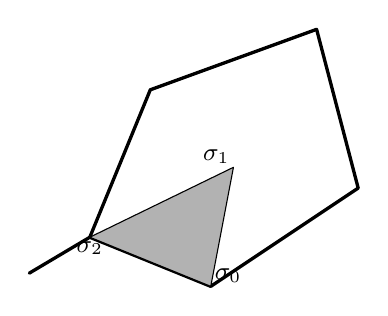
\begin{tikzpicture}[x=0.024cm,y=-0.024cm,line cap=round,line join=round,font=\small]
\coordinate (A) at (32,110);
\coordinate (B) at (64,32);
\coordinate (C) at (152,0);
\coordinate (D) at (174,84);
\coordinate (E) at (96,136);
\coordinate (O) at (108,73);
\coordinate (X) at (0,129);
\draw[very thick] (A)--(B)--(C)--(D);
\draw[very thick] (D)--(E);
\draw[very thick] (E)--(A);
\draw[very thick] (A)--(X);
\draw[fill=black!30] (A)--(O)--(E)--cycle;
\node[above left,inner sep=1.3pt] at (O) {$\sigma_{\unsure{1}}$};
\node[above right,inner sep=1.3pt] at (E) {$\sigma_0$};
\node[below,inner sep=1.3pt] at (A) {$\sigma_2$};
\end{tikzpicture}}

les $\bar\sigma_i$ engendrent $G$.

\margin{(Exer)}
% slanted

\uline{Proposition} Soit $\Pi$ \deleted{\unsure{polygone}}\unsure{polyèdre} \inserted{comb.} régulier connexe, $E=\operatorname{Rep}(\Pi)$, $G=\operatorname{Aut}(\Pi)$, $\Phi=$ ens des facettes de $\Pi$. --

a) Soit $p=\text{ordre}\,(\sigma_{\unsure{1}}\sigma_2)_E$, $q=\inserted{\text{ordre}}\,(\sigma_0\sigma_1)_E$. Alors par tt sommet de $\deleted{\unsure{E}}\Pi$ passent exact$^{\mathrm{t}}$ $p$ arêtes, \deleted{par} \inserted{sur} tte face il y a exact$^{\mathrm{t}}$ $q$ arêtes

(\uline{NB} $3\leq p,q\leq+\infty$).

b) Soit $s\in S(\Pi)$. Alors le hom du stabilisateur $G_s$ de \inserted{$s$ ds} $G$, dans $\operatorname{Aut}(\Phi_{\geq s})$ [ où $\Phi_{\geq s}$ est le polygône combinatoire à $p$ côtés

% archive sheet number: 15

